\chapter{Esperanza Matemática}

\section{Definición de Esperanza Matemática}


  Para una variable aleatoria discreta $X$ que toma valores $x_{1},...,x_{n},$ la \emph{esperanza matemática} se define como
  \begin{align}
   \label{eq:3.1}
   E(X)=\sum _{j=1}^{n} x_{j}P(X=x_{j})=:\sum xP(X=x),
  \end{align}

o de manera equivalente
  \begin{align}
   \label{eq:3.2}
   E(X)=\sum _{j=1}^{n} x_{j}f(x_{j})=:\sum xf(x),
  \end{align}
  donde $f(x)=P(X=x).$



 Como un caso especial, cuando $f(x)\equiv \frac{1}{n},$ obtenemos la \emph{media aritmética:}
 \begin{align}
  \label{eq:3.3}
  E(X)=\dfrac{\sum_{i=1}^{n}x_{i}}{n}.
 \end{align}


{}
\begin{ejemplo}
 Sea $X$ el número que se obtiene al lanzar un dado.  Entonces, cada cara $x$ tiene la misma probabilidad
 \begin{align*}
 f(x) = \frac{1}{6}
\end{align*} de caer.


Por tanto,
$E(X)= (1)\left( \frac{1}{6} \right)+...+(6)\left( \frac{1}{6} \right) = \dfrac{1+...+6}{6} = 3.5$
\end{ejemplo}



{Caso Discreto Numerable}
 En el caso en que $X$ tome un cantidad (infinita) numerable de valores $x_{1},x_{2},...,$ definimos
 \begin{align*}
  E(X)=\sum_{i=1}^{\infty}x_{i}f(x_{i}),
 \end{align*}
siempre y cuando dicha \emph{serie} converja.


% {}
% La serie anterior debe entenderse como el límite
% $\lim_{n\to \infty} \sum_{i=1}^{n} x_{i}f(x_{i}).$
%
%
% 

{Caso Continuo}
 Para una variable aleatoria continua $X$ que tenga función de densidad $f(x),$ la esperanza de $X$ se define como
 \begin{align}
  \label{eq:3.4}
  E(X)=\int_{-\infty}^{\infty}xf(x)dx
 \end{align}
siempre y cuando dicha \emph{integral} converja.


 La esperanza de $X$ es llamada a menudo \emph{media} de $X$ y es denotada por $\mu_{x},$ o simplemente $\mu,$ cuando la variable aleatoria subyacente se sobreentiende.


 La media o esperanza de $X$ da un único valor que representa el promedio de los valores de $X,$ y por esta razón decimos que es una \emph{medida de tendencia central.}



 \begin{ejemplo}
  \label{exmp:3.1}
  Supongamos que un juego se juega con un dado único que se suponen justos. En este juego, un jugador gana \$20 si un sale un $2$; \$40 con un $4$; \$30 con un $6$; y no gana ni pierde con cualquier otra cara. Encuentre la suma esperada de dinero que ganaría.
 \end{ejemplo}





 \begin{align*}
 \mu &= \$ 20 \left( \frac{1}{6} \right) + \$40 \left( \frac{1}{6} \right) + \$60\left( \frac{1}{6} \right) \\
   &= \dfrac{\$20 + \$40 + \$60 + 3\times\$ 0}{6} \\
   &= \$ 15
\end{align*}




 \begin{ejemplo}
  \label{exmp:3.2}
  La función de densidad de una variable aleatoria $X$ está dada por
  \begin{align*}
   f(x)=
   \begin{cases}
    \frac{1}{2}x & 0<x<2 \\
    0 & \texttt{en otro caso}
   \end{cases}
  \end{align*}
Encuentre el valor esperado de $X.$
 \end{ejemplo}



{}
\begin{align*}
 \mu &= E(X)\\ & = \int_{-\infty}^{\infty} xf(x) dx \\
  &= \int_{0}^{2} x\left( \dfrac{1}{2}x \right) dx\\
  &= \evat{\frac{1}{6} \, x^{3}}{0}{2}\\
  &= \frac{1}{6}(2)^{3}-\frac{1}{6}(0)^{3} \\
  &= \frac{4}{3}
\end{align*}


\subsection{Funciones de Variables Aleatorias}

 Sea $X$ una variable aleatoria discreta con función de probabilidad $f(x).$ Entonces $Y=g(X)$ es una variable aleatoria discreta con función de probabilidad
 \begin{align}
  h(y)=P(g(X)=y)=\sum_{\set{x|g(x)=y}}g(x)f(x)
 \end{align}



 Entonces, en el caso discreto.
 \begin{align}
 \label{eq:3.5}
  E\left( g(X) \right)=
  \sum_{x}g(x)f(x)
 \end{align}

 De manera similar, en el caso continuo
 \begin{align}
  \label{eq:3.6}
  E\left( g(X) \right)=\int_{-\infty}^{\infty}
  g(x)f(x)dx.
 \end{align}




 \begin{ejemplo}
  \label{exmp:3.3}
  Si $X$ es la variable aleatoria del ejemplo \ref{exmp:3.2}, encuentre $E\left( 3X^{2}-2X \right).$
 \end{ejemplo}


{}
En este caso, $g(x)=3x^2-2x.$



Recordemos que
  \begin{align*}
   f(x)=
   \begin{cases}
    \frac{1}{2}x & 0<x<2 \\
    0 & \texttt{en otro caso}
   \end{cases}
  \end{align*}



\begin{align*}
 E(3X^2-2X) &= E(g(X)) \\
  &= \displaystyle \int_{-\infty}^{\infty} \left( 3x^2-2x \right)f(x)dx\\
  &= \displaystyle \int_{0}^{2}\left( 3x^2-2x \right)\left( \dfrac{1}{2}x \right)dx \\
  &= \displaystyle \int_{0}^{2} \frac{3}{2} \, x^{3} - x^{2} dx
 \\  &= \displaystyle \evat{\frac{3}{8} \, x^{4} - \frac{1}{3} \, x^{3}
}{0}{2}
\\  &= \displaystyle
\frac{10}{3}
\end{align*}


\subsection{Algunos temas sobre esperanza matemática}
{Linealidad}
 \begin{thm}
  \label{thm:3.1}
  Si $c,d$ son constantes y $X,Y$ son variables aleatorias, entonces
  \begin{align}
   \label{linealidad}
   E\left( cX+dY \right)=
   cE\left( X \right)+dE\left( Y \right)
  \end{align}

 \end{thm}


{Esperanza e independencia}
 \begin{thm}
  \label{thm:3.3} Si $X,Y$ son \emph{variables aleatorias independientes}, entonces
  \begin{align}
   \label{eq:3.10}
   E\left( XY \right)=E(X)E(Y)
  \end{align}

 \end{thm}



\section{Varianza y Desviación Estándar}

 Ya vimos que la espereza matemática de una variable aleatoria $X$ es una medida de tendencia central y que generaliza a la \emph{media aritmética $\mu$.}
 

\begin{rem}
 Por esta razón, de aquí en adelante definiremos
 \begin{align*}
  \mu=\mu_{X}=E(X).
 \end{align*}

\end{rem}

 


 Otra cantidad de gran importancia es la \emph{varianza} que se define como
 \begin{align}
  \label{eq:3.11}
  \s_{X}^{2}=\Var(X)=E\left( \left( X-\mu_{X} \right)^{2} \right)
 \end{align}



 La \emph{desviación estándar} se definirá como
 \begin{align}
  \label{eq:3.12}
  \s_{X} = \sqrt{\Var{X}}
 \end{align}



 \begin{rem}
  Si la variable aleatoria $X$ se sobreentiende del contexto, omitiremos el subíndice correspondiente, es decir,
  \begin{align*}
   \mu=\mu_{X}, \; \s=\s_{X}, \; \s^{2}=\s_{X}^{2}.
  \end{align*}

 \end{rem}



 Si $X$ es una variable aleatoria discreta, la varianza está dada por
 \begin{align}
  \label{eq:3.13}
  \s^{2}=E\left( \left( X-\mu \right)^{2} \right)=\sum\left( x-\mu \right)^{2}f(x),
 \end{align}
 siempre y cuando esta suma converja.


En el caso de que todas las probabilidades sean iguales y la variable aleatoria $X$ sea finita tenemos
\begin{align}
\label{eq:3.14}
 \s^{2}=\dfrac{\left( x_{1}-\mu \right)^{2}+...+\left( x_{n}-\mu \right)^{2} }{n}
\end{align}



{}
\begin{ejemplo}
 Como vimos anteriormente, si $X$ es la cara obtenida al lanzar un dado, entonces $\mu_{X}=3.5$.


La varianza de $X$ es
\begin{align*}
 \s^{2}
 &= \displaystyle \dfrac{(1-3.5)^2+...+(6-3.5)^2}{6}
 \\  &= \displaystyle \frac{17.5}{6}
 \\  &\approx \displaystyle 2.916
\end{align*}
\end{ejemplo}




 Si $X$ es una variable aleatoria continua con función de densidad $f(x),$ entonces la varianza está dada por
 \begin{align}
  \label{eq:3.15}
  \s^{2}=E\left( (X-\mu)^{2} \right)=
  \int_{-\infty}^{\infty}\left( x-\mu \right)^{2}f(x)dx
 \end{align}
siempre y cuando la integral converja.


 Tanto la varianza como la desviación estándar es una \emph{medida de dispersión.}
 \begin{figure}[h]
 \centering
 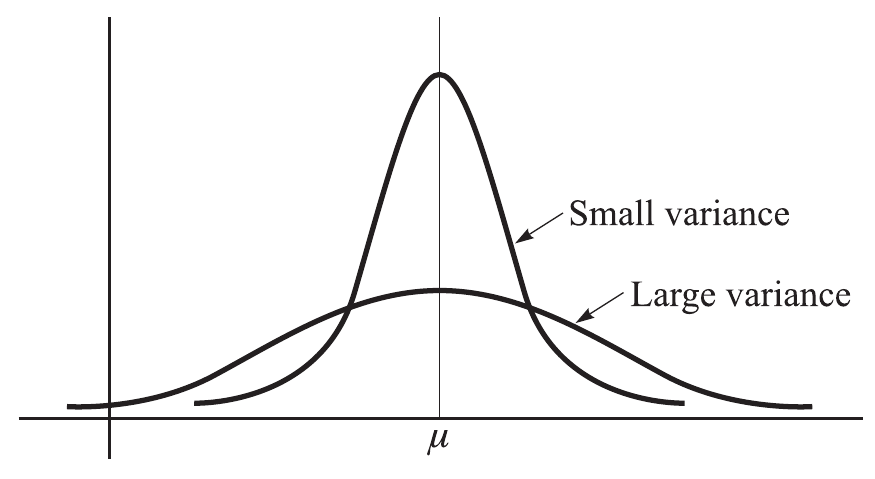
\includegraphics[height=5cm,keepaspectratio=true]{./pe/pands0301.png}
 % pands0301.png: 0x0 pixel, 300dpi, 0.00x0.00 cm, bb=
 \label{fig:0301}
\end{figure}



 \begin{ejemplo} %falta escribir esto en la libreta
  \label{exmp:3.4}
  Encuentre la varianza y la desviación estándar de la variable aleatoria del ejemplo \ref{exmp:3.2}.
 \end{ejemplo}


{}
Recordemos que esta variable aleatoria $X$ tiene densidad de probabilidad
  \begin{align*}
   f(x)=
   \begin{cases}
    \frac{1}{2}x & 0<x<2 \\
    0 & \texttt{en otro caso}
   \end{cases}
  \end{align*}

{}
\begin{align*}
 \sigma^2 = Var(X) &= \displaystyle \int_{0}^{2}(x-\frac{4}{3})^2f(x) dx
 \\  &= \displaystyle \int_{0}^{2} \frac{1}{2} \, {\left(x - \frac{4}{3}\right)}^{2} x dx
 \\  &= \displaystyle
 \evat{\frac{1}{8} \, x^{4} - \frac{4}{9} \, x^{3} + \frac{4}{9} \, x^{2}}{0}{2}
 \\  &= \displaystyle \frac{2}{9}
\\  &\approx \displaystyle 0.\bar{2}
\end{align*}

{Algunos teoremas sobre Varianza}
\begin{align}
 \label{eq:3.16}
 \s^{2}=E\left( X^{2} \right)-\mu^{2} \\ 
 \label{eq:3.17}
 \Var\left( cX \right)=c^{2}\Var\left( X \right)\\ 
 \label{thm:3.6}
 \s^{2}=\min_{a}\set{E\left( \left( X-a \right)^{2} \right)}
\end{align}

Si $X,Y$ son independientes
\begin{align}
 \label{eq:3.18}
 \Var(X\pm Y)=\Var(X)+\Var(Y)
\end{align}


{Variables Aleatorias Estandarizadas}
 Sea $X$ una variable aleatoria con media $\mu$ y desviación estándar $\s>0.$ Diremos que la \emph{variable aleatoria estandarizada} asociada está dada por
 \begin{align}
  \label{eq:3.20}
  X^{*}=\dfrac{X-\mu}{\s}.
 \end{align}


\begin{align}
 \label{eq:3.21}
 E\left( X^{*} \right)=0, \; \Var(X^{*})=1.
\end{align}


\section{Covarianza y correlación}

Los resultados dados anteriormente para una variable aleatoria pueden extenderse a dos variables.


{}

\begin{equation}
 \label{eq:3.43}
 \begin{split}
  \mu_{X}=E(X)=\int_{-\infty}^{\infty}\int_{-\infty}^{\infty} xf(x,y)dxdy\\ 
  \mu_{Y}=E(Y)=\int_{-\infty}^{\infty}\int_{-\infty}^{\infty}
  yf(x,y)dxdy
 \end{split}
\end{equation}





\begin{equation}
 \label{eq:3.44}
 \begin{split}
  \s^{2}_{X}=E\left( (X-\mu_{X})^{2} \right)=\int_{-\infty}^{\infty}\int_{-\infty}^{\infty} (x-\mu_{X})^2f(x,y)dxdy\\ 
  \s^{2}_{Y}=E\left( (Y-\mu_{Y})^{2} \right)=\int_{-\infty}^{\infty}\int_{-\infty}^{\infty} (y-\mu_{Y})^2f(x,y)dxdy
 \end{split}
\end{equation}


{Covarianza}
 \begin{align}
 \label{eq:3.45}
  \s_{XY}=\cov(X,Y)=E\left( (X-\mu_{X})(Y-\mu_{Y}) \right)
 \end{align}



 \begin{align}
  \label{eq:3.46}
  \s_{XY}=\int_{-\infty}^{\infty}
  \int_{-\infty}^{\infty}
  (x-\mu_{X})(y-\mu_{Y})f(x,y)dxdy
 \end{align}


{Caso Discreto}

 \begin{equation}
  \begin{split}
   \mu_{X}=\sum_{x}\sum_{y}xf(x,y) \\
  \mu_{Y}=\sum_{x}\sum_{y}yf(x,y)
  \end{split}
 \end{equation}



 \begin{align}
  \label{eq:3.48}
  \s_{XY}=\sum_{x}\sum_{y}(x-\mu_{X})(y-\mu_{Y})f(x,y)
 \end{align}



 \begin{align}
  \label{eq:3.50}
  \s_{XY}=E(XY)-E(X)E(Y)=E(XY)-\mu_{X}\mu_{Y}
 \end{align}


 Si $X,Y$ son independientes, entonces
 \begin{align}
  \label{eq:3.50}
  \s_{XY}=\cov(X,Y)=0
 \end{align}



 \begin{align}
  \label{eq:3.51}
  \Var(X\pm Y)=\Var(X)\pm2\cov(X,Y)+\Var(Y).
 \end{align}




 De manera equivalente,
 \begin{align}
  \label{eq:3.52}
  \s_{X\pm Y}^{2}=\s_{X}^{2} \pm 2\s_{XY} +\s_{Y}^{2}
 \end{align}


{Coeficiente de correlación de Pearson}
 \begin{align}
  \label{eq:3.54}
  \rho = \dfrac{\s_{XY}}{\s_{X}\s_{Y}}
 \end{align}



 \begin{thm}
  \begin{align}
   \label{eq:3.53}
   \abs{\s_{XY}}\leq \s_{X}\s_{Y}
  \end{align}


 \begin{align}
  \abs{\rho}\leq 1.
 \end{align}
 \end{thm}


{Propiedades de la correlación}

\begin{enumerate}
\item $-1 \leq \rho \leq 1$ 
 \item $\rho \approx 0$: \emph{Correlación débil}, prácticamente no existe una correlación lineal. 
 \item $\abs{\rho} \approx 1$:\emph{ Correlación fuerte}, la correlación está dada prácticamente por una función afín $y=mx+b$. 
 \item $\rho > 0$: \emph{Correlación positiva}, en la medida que una crece, la otra también crece. 
 \item $\rho < 0$: \emph{Correlación negativa}, en la medida que una crece, la otra decrece.
\end{enumerate}



 \begin{ejemplo}
  \label{sol:3.25}
  \emph{Sean $X,Y$ variables aleatorias discretas} con densidad de probabilidad conjunta
  \begin{align}f(x,y)=
   \begin{cases}
    \dfrac{2x+y}{42} & 0\leq x \leq 2,\; 0\leq y \leq 3 \\
    0 & \texttt{en otro caso}.
   \end{cases}
  \end{align}
 \end{ejemplo}
 

Encuentre los siguientes estadísticos:
\begin{multicols}{3}
 \begin{enumerate}[(a)]
 \item $\mu_X = E(X)$ %
 \item $\mu_Y = E(Y)$ %
 \item $ E(XY)$ %
 \item $E(X^2)$ %
 \item $E(Y^2)$ %
 \item $\s^2_X = \Var(X)$ %
 \item $\s_{Y}$
 \item $\s^2_Y = \Var(Y)$ %
 \item $\s_{Y}$
 \item $\s_{XY} =\cov(X,Y)$ %
 \item $\rho$
\end{enumerate}
\end{multicols}






 \begin{ejemplo}
  \label{sol:3.26}
  \emph{Sean $X,Y$ variables aleatorias continuas} con densidad de probabilidad conjunta
  \begin{align}f(x,y)=
   \begin{cases}
    \frac{1}{210}(2x+y) & 2 < x < 6,\; 0<y<5 \\
    0 & \texttt{en otro caso}.
   \end{cases}
  \end{align}
 \end{ejemplo}

 

Encuentre los siguientes estadísticos:
\begin{multicols}{3}
 \begin{enumerate}[(a)]
 \item $\mu_X = E(X)$ %
 \item $\mu_Y = E(Y)$ %
 \item $ E(XY)$ %
 \item $E(X^2)$ %
 \item $E(Y^2)$ %
 \item $\s^2_X = \Var(X)$ %
 \item $\s_{Y}$
 \item $\s^2_Y = \Var(Y)$ %
 \item $\s_{Y}$
 \item $\s_{XY} =\cov(X,Y)$ %
 \item $\rho$
\end{enumerate}
\end{multicols}




